% Generated from Graphviz DOT by figures/make_figures.py; do not edit by hand.
\definecolor{slateink}{HTML}{334155}
\definecolor{slateedge}{HTML}{475569}
\definecolor{slatemid}{HTML}{64748B}
\definecolor{slatefill}{HTML}{F8FAFC}
\definecolor{orangefill}{HTML}{FFF7ED}
\definecolor{orangeedge}{HTML}{C2410C}
\definecolor{redfill}{HTML}{FEE2E2}
\definecolor{rededge}{HTML}{DC2626}
\definecolor{bluefill}{HTML}{DBEAFE}
\definecolor{blueedge}{HTML}{2563EB}
\definecolor{greenfill}{HTML}{DCFCE7}
\definecolor{greenedge}{HTML}{16A34A}
\definecolor{greenlight}{HTML}{F0FDF4}
\definecolor{greendark}{HTML}{15803D}
\definecolor{indigofill}{HTML}{EEF2FF}
\definecolor{indigoedge}{HTML}{4F46E5}
\definecolor{cyanfill}{HTML}{ECFEFF}
\definecolor{cyanedge}{HTML}{0891B2}
\definecolor{slatefillb}{HTML}{F1F5F9}
\definecolor{purplefill}{HTML}{FAE8FF}
\definecolor{purpleedge}{HTML}{A21CAF}
\definecolor{amberfill}{HTML}{FFFBEB}
\definecolor{amberedge}{HTML}{B45309}
\definecolor{pinkfill}{HTML}{FFF1F2}
\definecolor{bluelight}{HTML}{EFF6FF}
\definecolor{amberfillb}{HTML}{FEF3C7}
\definecolor{amberedgeb}{HTML}{D97706}
\definecolor{skyfill}{HTML}{E0F2FE}
\definecolor{skyedge}{HTML}{0284C7}
\definecolor{yellowfill}{HTML}{FEF9C3}
\definecolor{yellowedge}{HTML}{CA8A04}
\definecolor{orangefillb}{HTML}{FFEDD5}
\definecolor{orangeedgeb}{HTML}{EA580C}
\definecolor{grayfill}{HTML}{E2E8F0}
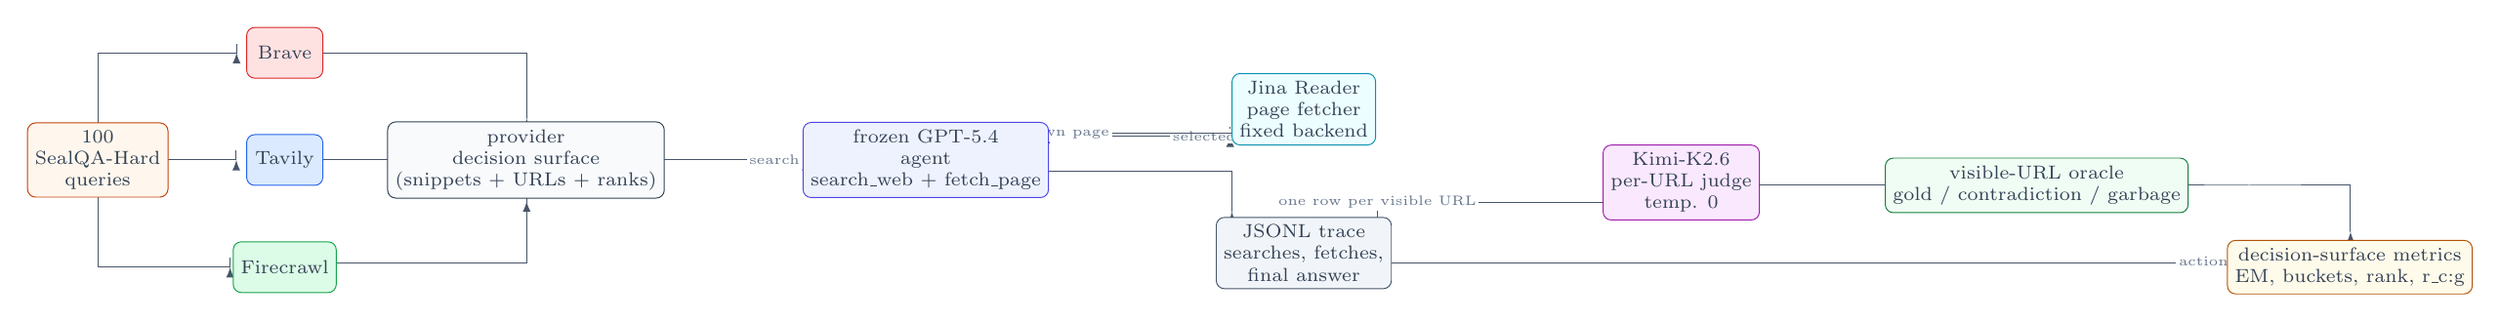
\begin{tikzpicture}[x=0.52in,y=0.52in,>=latex]
\tikzset{gvnode/.style={draw, rounded corners=3pt, align=center, font=\scriptsize, inner sep=2.8pt, line width=0.35pt}}
\tikzset{gvedge/.style={->, line width=0.35pt, color=slateedge}}
\draw[gvedge] (0.583,1.686) -- (0.583,1.997) -- (0.583,2.431) -- (0.583,2.431) -- (0.583,2.431) -- (1.950,2.431) -- (1.950,2.431);
\draw[gvedge] (1.171,1.375) -- (1.171,1.375) -- (1.947,1.375) -- (1.947,1.375);
\draw[gvedge] (0.583,1.064) -- (0.583,0.753) -- (0.583,0.319) -- (0.583,0.319) -- (0.583,0.319) -- (1.886,0.319) -- (1.886,0.319);
\draw[gvedge] (2.801,2.431) -- (3.473,2.431) -- (4.806,2.431) -- (4.806,2.431) -- (4.806,2.431) -- (4.806,1.783) -- (4.806,1.783);
\draw[gvedge] (2.800,1.375) -- (2.800,1.375) -- (3.583,1.375) -- (3.583,1.375);
\draw[gvedge] (2.866,0.361) -- (3.555,0.361) -- (4.806,0.361) -- (4.806,0.361) -- (4.806,0.361) -- (4.806,0.968) -- (4.806,0.968);
\draw[gvedge] (5.922,1.375) -- (5.922,1.375) -- (7.555,1.375) -- (7.555,1.375);
\node[font=\tiny, fill=white, inner sep=1pt, text=slatemid] at (7.555,1.375) {search surface};
\draw[gvedge] (9.823,1.607) -- (9.823,1.607) -- (11.733,1.607) -- (11.733,1.607);
\node[font=\tiny, fill=white, inner sep=1pt, text=slatemid] at (11.733,1.607) {selected URLs};
\draw[gvedge] (9.820,1.264) -- (10.684,1.264) -- (11.750,1.264) -- (11.750,1.264) -- (11.750,1.264) -- (11.750,0.865) -- (11.750,0.865);
\draw[gvedge] (11.831,1.643) -- (11.831,1.643) -- (9.920,1.643) -- (9.920,1.643);
\node[font=\tiny, fill=white, inner sep=1pt, text=slatemid] at (9.920,1.643) {markdown page};
\draw[gvedge] (13.181,0.766) -- (13.181,0.869) -- (13.181,0.958) -- (13.181,0.958) -- (13.181,0.958) -- (15.442,0.958) -- (15.442,0.958);
\node[font=\tiny, fill=white, inner sep=1pt, text=slatemid] at (13.181,0.958) {one row per visible URL};
\draw[gvedge] (13.266,0.361) -- (13.266,0.361) -- (21.623,0.361) -- (21.623,0.361);
\node[font=\tiny, fill=white, inner sep=1pt, text=slatemid] at (21.623,0.361) {actions + EM};
\draw[gvedge] (16.807,1.125) -- (16.807,1.125) -- (18.345,1.125) -- (18.345,1.125);
\draw[gvedge] (20.904,1.125) -- (21.766,1.125) -- (22.764,1.125) -- (22.764,1.125) -- (22.764,1.125) -- (22.764,0.667) -- (22.764,0.667);
\node[gvnode, minimum width=0.607in, minimum height=0.318in, fill=orangefill, draw=orangeedge, text=slateink] (q) at (0.583,1.375) {100\\SealQA-Hard\\queries};
\node[gvnode, minimum width=0.390in, minimum height=0.260in, fill=redfill, draw=rededge, text=slateink] (brave) at (2.424,2.431) {Brave};
\node[gvnode, minimum width=0.390in, minimum height=0.260in, fill=bluefill, draw=blueedge, text=slateink] (tavily) at (2.424,1.375) {Tavily};
\node[gvnode, minimum width=0.455in, minimum height=0.260in, fill=greenfill, draw=greenedge, text=slateink] (firecrawl) at (2.424,0.319) {Firecrawl};
\node[gvnode, minimum width=1.163in, minimum height=0.318in, fill=slatefill, draw=slateink, text=slateink] (surface) at (4.799,1.375) {provider\\decision surface\\(snippets + URLs + ranks)};
\node[gvnode, minimum width=1.127in, minimum height=0.318in, fill=indigofill, draw=indigoedge, text=slateink] (agent) at (8.736,1.375) {frozen GPT-5.4\\agent\\search\_web + fetch\_page};
\node[gvnode, minimum width=0.650in, minimum height=0.318in, fill=cyanfill, draw=cyanedge, text=slateink] (jina) at (12.458,1.875) {Jina Reader\\page fetcher\\fixed backend};
\node[gvnode, minimum width=0.838in, minimum height=0.318in, fill=slatefillb, draw=slateedge, text=slateink] (trace) at (12.458,0.458) {JSONL trace\\searches, fetches,\\final answer};
\node[gvnode, minimum width=0.657in, minimum height=0.318in, fill=purplefill, draw=purpleedge, text=slateink] (judge) at (16.174,1.153) {Kimi-K2.6\\per-URL judge\\temp. 0};
\node[gvnode, minimum width=1.278in, minimum height=0.260in, fill=greenlight, draw=greendark, text=slateink] (oracle) at (19.674,1.125) {visible-URL oracle\\gold / contradiction / garbage};
\node[gvnode, minimum width=1.076in, minimum height=0.260in, fill=amberfill, draw=amberedge, text=slateink] (metrics) at (22.757,0.319) {decision-surface metrics\\EM, buckets, rank, r\_c:g};
\end{tikzpicture}
